% Theoretical background
%\clearpage%if the chapter heading starts close to bottom of the page, force a
% line break and remove the vertical vspace
\vspace{21.5pt}
\chapter{Analysis: Current vs. Proposed}
In this chapter, a detailed comparison is provided to highlight the differences
and improvements from incorporating fuzzy testing into existing system workflows.
The main goal is to study the current, then proposed workflow. This outlines the
fuzzy testing method in software development and testing. Each step of the workflow
is closely examined, comparing current practices with the potential enhancements
brought about by integrating fuzzy testing. The Table:~\ref{tab:system_workflows_comparison_fuzzy}
and Figure:~\ref{fig:simplified_workflow_proposed} offer a clear visual representation,
outlining the impact of fuzzy testing on the \acrlong{sdlc}

\section{Embedded System With Root Of Trust Architecture}
Reflecting on the prior discussions of embedded systems in
Section~\ref{sec:sec_introduction} and Section~\ref{sec:embedded_system} respectively,
this chapter explores current state analysis of the case in company and proposed
state of analysis with respect to fuzzing.

In an increasingly digital and interconnected world, the security of
embedded systems is paramount. Embedded systems, ranging from tiny
\gls{iot} devices to large-scale industrial control
systems, form the backbone of modern infrastructure. However,
their pervasiveness also makes them a tempting target for attackers. Vulnerabilities such as
Meltdown\cite{lipp2020meltdown} and Spectre\cite{kocher2020spectre} are some recent examples.

The Figure:~\ref{fig:rot} illustrates high-level depiction of the architecture for
the case in company.

\begin{figure}[H]
    \centering
    \AltText{Diagram illustrating the Embedded Root of Trust Architecture,
    highlighting the core components such as secure boot, trusted execution
    environment, cryptographic operations, and hardware-based key storage. The
    architecture is depicted as a layered structure, emphasizing the
    foundational role of trust in secure embedded systems.}
    {\adjustbox{width=\textwidth}{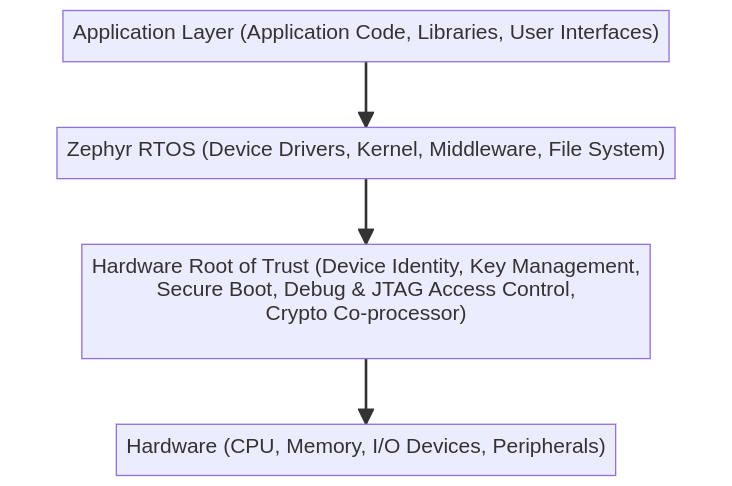
\includegraphics{illustration/RoT.png}}}
    \caption{Embedded Root of Trust Architecture\cite{Introduc82:online}}\label{fig:rot}
\end{figure}


% \begin{figure}[ht]
%         \centering
%         \AltText{Embedded Root of Trust Architecture}{\includegraphics[width=9.5cm, height=10.5cm]{rot}}
%         \caption{Embedded Root of Trust Architecture}\label{fig:rot}
% \end{figure}


\textbf{Hardware:} This represents the physical components and sub-systems compromise
\gls{cpu}, memory~\cite{WhatisCo30:online} and other peripherals. It acts as a base layer on which
rest of the system operates.

\textbf{Hardware Root of Trust:} Roots of Trust refer to secure components within a computer system,
encompassing hardware, software, or firmware~\cite{WhatIsFi49:online}, that carry out crucial
security operations like data encryption, certificate validation and key management~\cite{RootofTr86:online}.
This is a principle that initiates a trust sequence, which is essential for verifying that
computers start up using authentic code. They serve as the foundational elements upon which the
security of other system components is established. Given their critical role, these elements must
be designed with a high level of
security~\cite{WhatisRo39:online}~\cite{RootofTr86:online}.

\textit{Hardware Root of Trust} ensures the integrity of the lower level system operations such as
secure boot\cite{zimmer2016establishing}, Debug and JTAG access control, Key management and Crypto Co-processors.
The \textit{secure boot} is a mechanism that the system uses to ensure that it ``boots'' in a known secure state.
The \acrshort{rot} plays a critical role in this process, verifying the integrity of the boot firmware and
subsequently loaded software~\cite{zimmer2016establishing}.

The \textit{debug and JTAG access control} needs careful handling as it can be used maliciously although
an essential feature for debugging and troubleshooting purpose~\cite{WhatisJT98:online}~\cite{JTAGhard62:online}.

The \textit{device identity and key management} component helps in ensuring the use, storage
and generation of cryptographic keys. A unique identification is assigned to each device
in the system for authentication. Key management typically involves a \gls{hsm} for storage
of the keys~\cite{WhatisKe81:online}. The keys are used for different operations such
as encryption~\cite{WhatisEn13:online}, signing, and authentication~\cite{needham1978using}.

The \textit{crypto core} is a component used in the \gls{rot} implementations
designed to be resistant to attack. This usually isolated from rest of the devices, helps
to protect the crypto core from being compromised. Some of the common cryptographic functions
are AES~\cite{nechvatal2001report}, RSA~\cite{milanov2009rsa}, and ECC~\cite{bos2014elliptic}.

\textbf{Zephyr RTOS\cite{Security75:online}~\cite{ZephyrPr4:online}~\cite{ZephyrPr92:online}}
serves as a vital bridge between the hardware and application layers in an embedded system.
This compact, open-source Real-Time Operating System (RTOS) is thoughtfully engineered for devices
with resource limitations. Zephyr RTOS plays a critical role in facilitating the Root of Trust (RoT)
functionalities, such as secure boot, cryptographic procedures,
and device validation\cite{Security75:online}~\cite{ZephyrPr4:online}~\cite{ZephyrPr92:online}.

Key elements within the Zephyr RTOS include:
\begin{enumerate}
\item Device Drivers: The device drivers play a significant role in bringing the hardware
components, necessary for the Root of Trust, into operation. These hardware components
could be the cryptographic engine or the secure boot bootloader~\cite{Bootload40:online}. Besides initialization,
these drivers make it possible for the kernel to manage and command these devices.
\item Kernel~\cite{Kernelin72:online}: The kernel acts as the system's core, ensuring that only verified software is allowed
to boot up on the device. Its role is critical in maintaining the security condition
of the device, by managing processes, task scheduling, memory, and inter-process communication.
\item Middleware: This component offers a range of security services including secure storage
solutions for cryptographic keys and secure transmission protocols. It essentially forms a bridge
between applications and the underlying network services.
\item File System: The file system is employed to safeguard the security configuration
of the device, along with other classified information. Its main function is to prevent
unauthorized access or tampering with this sensitive data.
\end{enumerate}
Together, these components within the Zephyr RTOS form the backbone of a secure, robust RoT,
offering a trustworthy platform for all software operations within the system.

\textbf{Application Layer} includes the end-user applications, libraries, and
user interfaces. It interacts with the Zephyr RTOS to perform its operations. It provides the
important security features for the users.

\section{Current Workflow for Embedded Software Systems}
In the case company, the development and deployment of embedded software systems
follow a structured workflow, encompassing stages such as design, development,
testing, and deployment in a continuous process. This workflow ensures a comprehensive approach from the
initial idea to the final real-world application. Subsequent sections will delve
into each stage in detail, highlighting their vital role in creating dependable
and efficient embedded software solutions.

\subsection*{Development Environment and Version Control:} Using
Git~\cite{loeliger2012version} provides a clear path through the software
development lifecycle. Gerrit~\cite{milanesio2013learning}, used for hosting
repositories, ensures a thorough review for every code change, contributing to
consistent and quality code.

The Figure:~\ref{fig:CI_Infrastrcuture_2} presents the IT infrastructure of CI/CD
flow for the company.

\begin{figure}[H] \centering
\AltText{Comprehensive diagram of the case company's
Embedded CI/CD (Continuous Integration/Continuous Deployment) Workflow,
illustrating a sequence of stages from code integration, automated testing,
to deployment in an embedded system environment. The workflow highlights the
integration of development, testing, and deployment processes for
efficient software delivery.}
{\adjustbox{width=\textwidth}{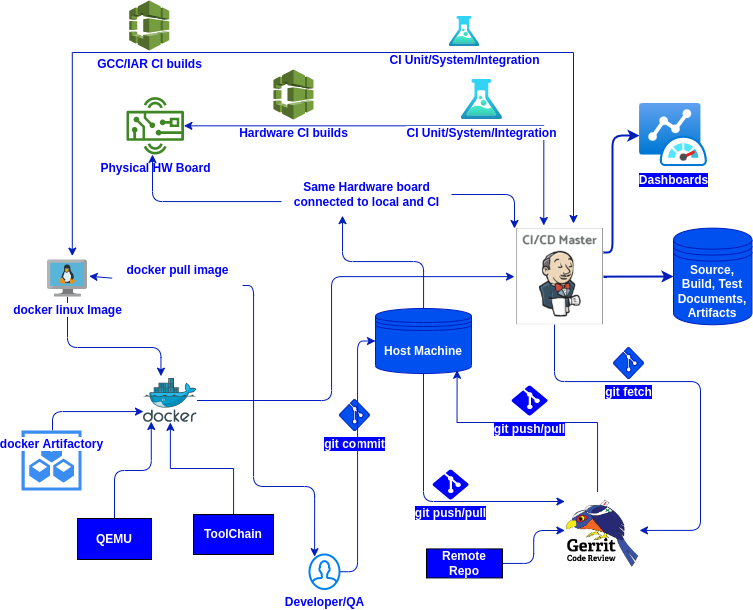
\includegraphics{CI_Infrastrcuture_2}}}
\caption{Embedded CI/CD Workflow}\label{fig:CI_Infrastrcuture_2} \end{figure}

\subsection*{Using Docker for Environment Consistency and QEMU:} To maintain a
consistent development environment, Docker~\cite{anderson2015docker} containers
are utilized to package necessary dependencies for the Zephyr RTOS firmware
compilation, reducing discrepancies during builds. QEMU~\cite{bellard2005qemu},
as a hardware emulator, enables testing in a simulated environment, which is
crucial for early detection of potential issues.

The Docker image~\cite{bui2015analysis} with QEMU is then stored in the JFrog
Artifactory~\cite{Artifact8:online} for use by developers.

\subsection*{Compilation Builds with GCC and IAR:} Different compiler
configurations are essential to cater to varied needs.
GCC~\cite{GCCtheGN9:online}, known for its practicality, offers a suite of compilers for different
programming languages. Conversely, IAR~\cite{AboutIAR98:online} provides
specialized compilers for embedded systems, aiming for optimal performance and
smaller footprints, which are vital for resource-constrained devices. Both
compilers ensure the Zephyr RTOS firmware is compatible across diverse platforms.

Automated processes compile the code post-modification, utilizing tools such as
Clang Static Analyzer~\cite{kremenek2008finding} and
Coverity~\cite{imtiaz2019developers} for static analysis to identify potential
issues.

\subsection*{Testing Frameworks:}

Ztest~\cite{TestFram11:online}, also known as the Zephyr Test Framework,
is a unit testing framework~\cite{runeson2006survey}
designed to validate the correctness of individual segments of Zephyr RTOS
code~\cite{TestFram11:online}.

The Pytest framework~\cite{hunt2019pytest}, on the other hand, examines the
overall functionality and interactions between the system's components, serving
as a tool for system and integration testing~\cite{TheFourL21:online}.

\textbf{Deployment and Continuous Monitoring:}

Jenkins~\cite{jenkins1963jenkins}, a renowned continuous integration tool~\cite{smart2011jenkins}, manages
various essential operations within the development
workflow~\cite{sayfan2017mastering}. Each code submission to the repository~\cite{milanesio2013learning}
initiates a series of processes including code compilation, unit testing~\cite{runeson2006survey} with
Ztest framework~\cite{TestFram11:online}, and system and integration
testing~\cite{TheFourL21:online} via the Pytest framework~\cite{hunt2019pytest}.
Developers are promptly informed of any issues detected during the build or test
stages.

The Jenkins interface offers detailed dashboards showcasing metrics like
instances of build failure and processing times. Moreover, extensive reports are
archived for future analysis. Continuous monitoring post-deployment is vital to
ensure the firmware's steady and efficient functioning~\cite{mcallister2015mastering}.
\pagebreak

\subsection{Simplified Current Workflow}

The Figure:~\ref{fig:simplified_workflow_current} illustrates further simplified depiction of the
current workflow~\ref{fig:CI_Infrastrcuture_2} used in the case company.

% \begin{figure}[H]
%         \centering
%         \adjustbox{width=\textwidth}{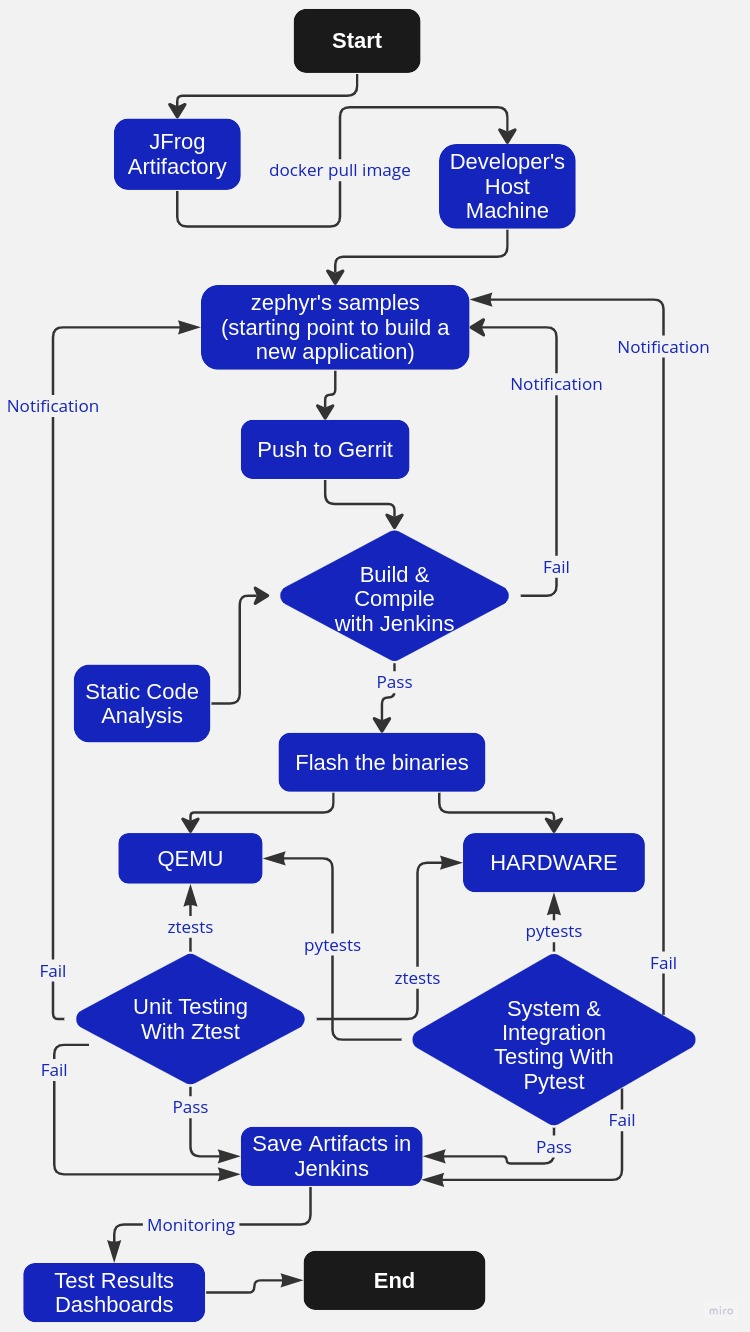
\includegraphics{simplified_workflow_current}}
%         \caption{Simplified Current Workflow}\label{fig:simplified_workflow_current}
% \end{figure}
% \begin{figure}[H]
%         \centering
%         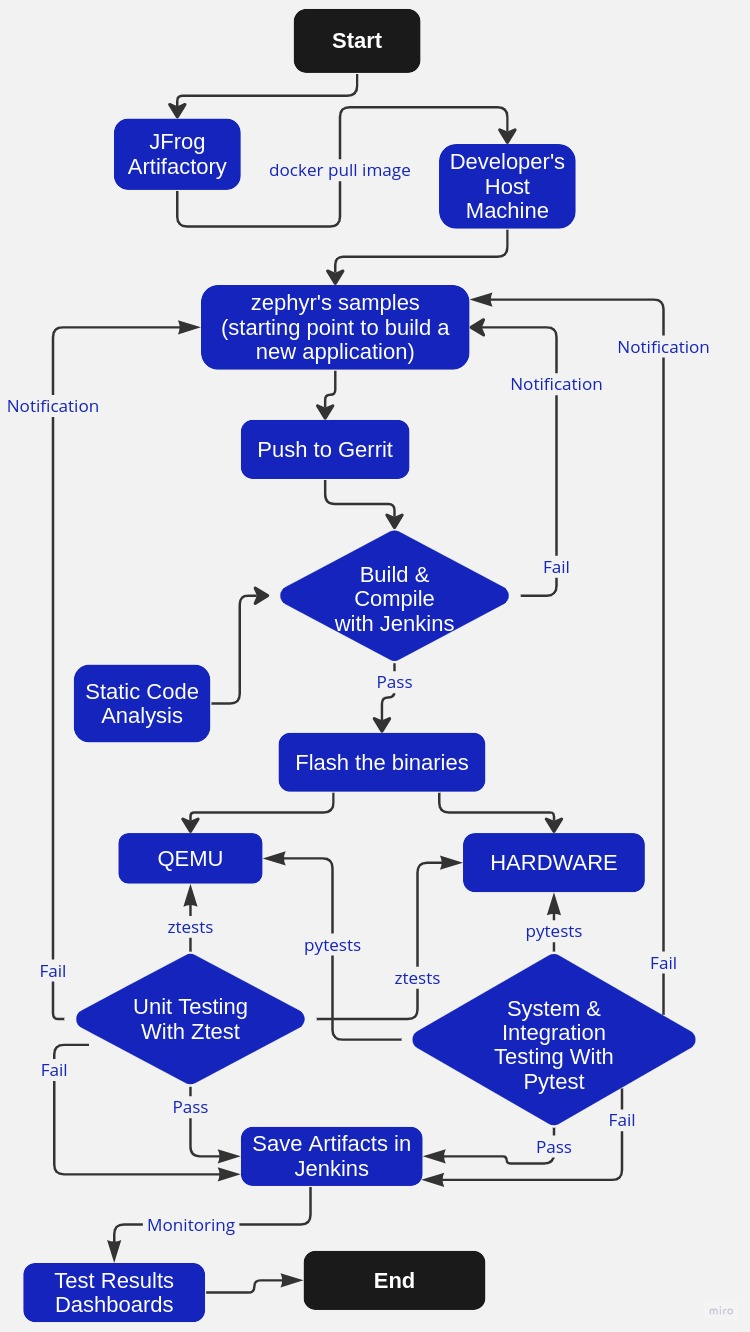
\includegraphics[width=\textwidth]{simplified_workflow_current}
%         \caption{Simplified Current Workflow}
%         \label{fig:simplified_workflow_current}
%     \end{figure}

\begin{figure}[H]
\centering
\AltText{Flow diagram of the Simplified Current Workflow, outlining the key
steps in a sequential manner, including initial planning, development,
testing, and deployment phases. The diagram emphasizes a linear and
efficient process flow, highlighting critical decision points and
transitions between stages.}
{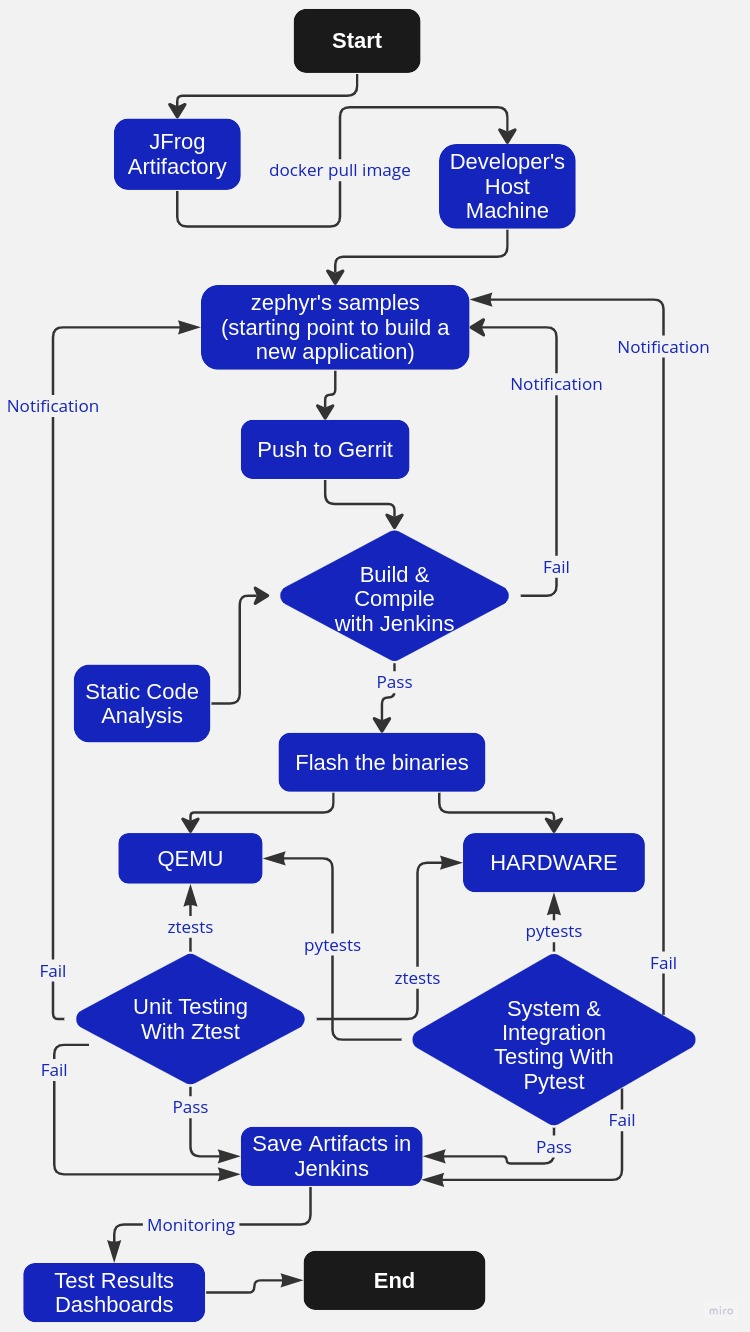
\includegraphics[width=\textwidth,height=0.8\textheight,keepaspectratio]{simplified_workflow_current}}
\caption{Simplified Current Workflow}
\label{fig:simplified_workflow_current}
\end{figure}

\section{Proposed Workflow With Fuzzing}
In light of the previously detailed current analysis, it becomes imperative to
explore enhancements that could further fortify the software development
lifecycle. One such augmentation revolves around the incorporation of
fuzzing, thereby aiming to unearth vulnerabilities
that conventional testing approaches might overlook.

The Figure:~\ref{fig:simplified_workflow_proposed} illustrates a simplified depiction of the
proposed workflow used in the case company.
\begin{figure}[H]
\centering
\AltText{Flow diagram of the Enhanced Workflow, building upon the Simplified
Current Workflow with the integration of fuzzing. The diagram shows standard
workflow steps like planning, development, and testing, with fuzzing added as a
key stage in the testing phase to improve security and identify vulnerabilities.}
{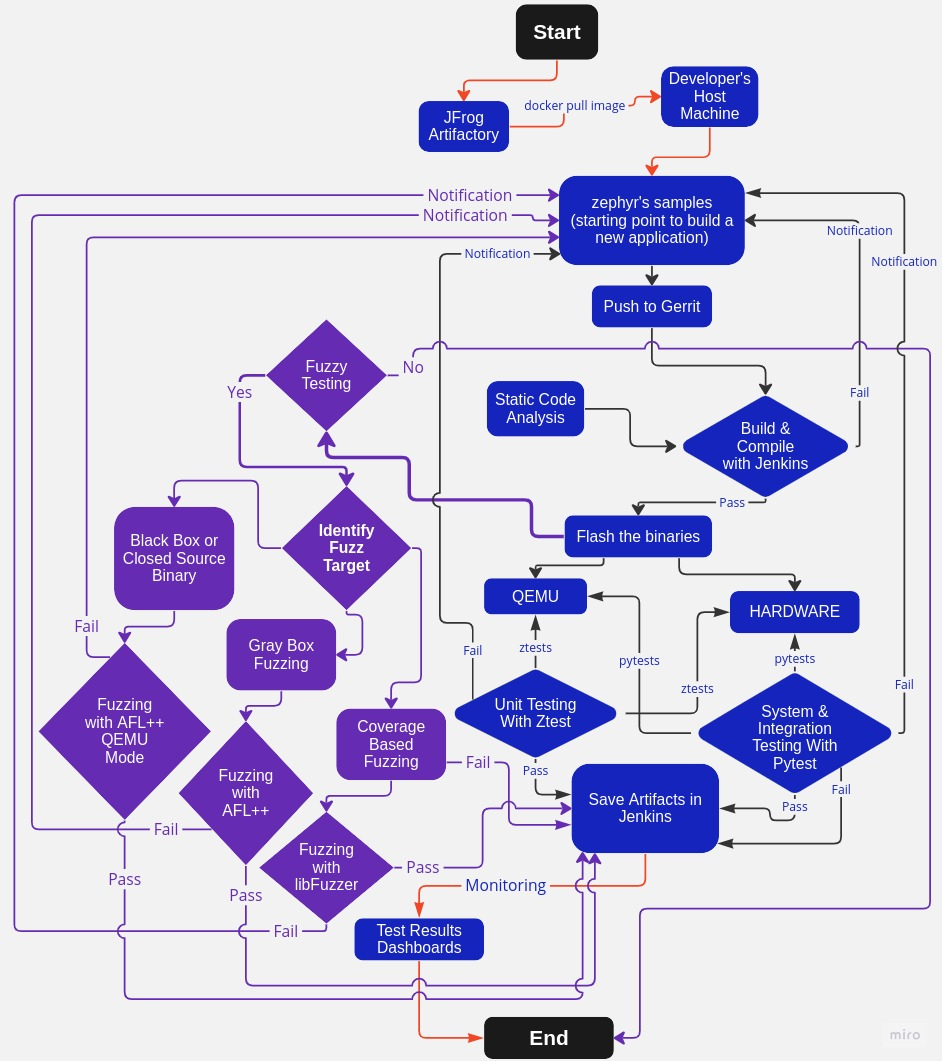
\includegraphics[width=\textwidth,height=0.8\textheight,keepaspectratio]{fuzzy_current_proposed}}
%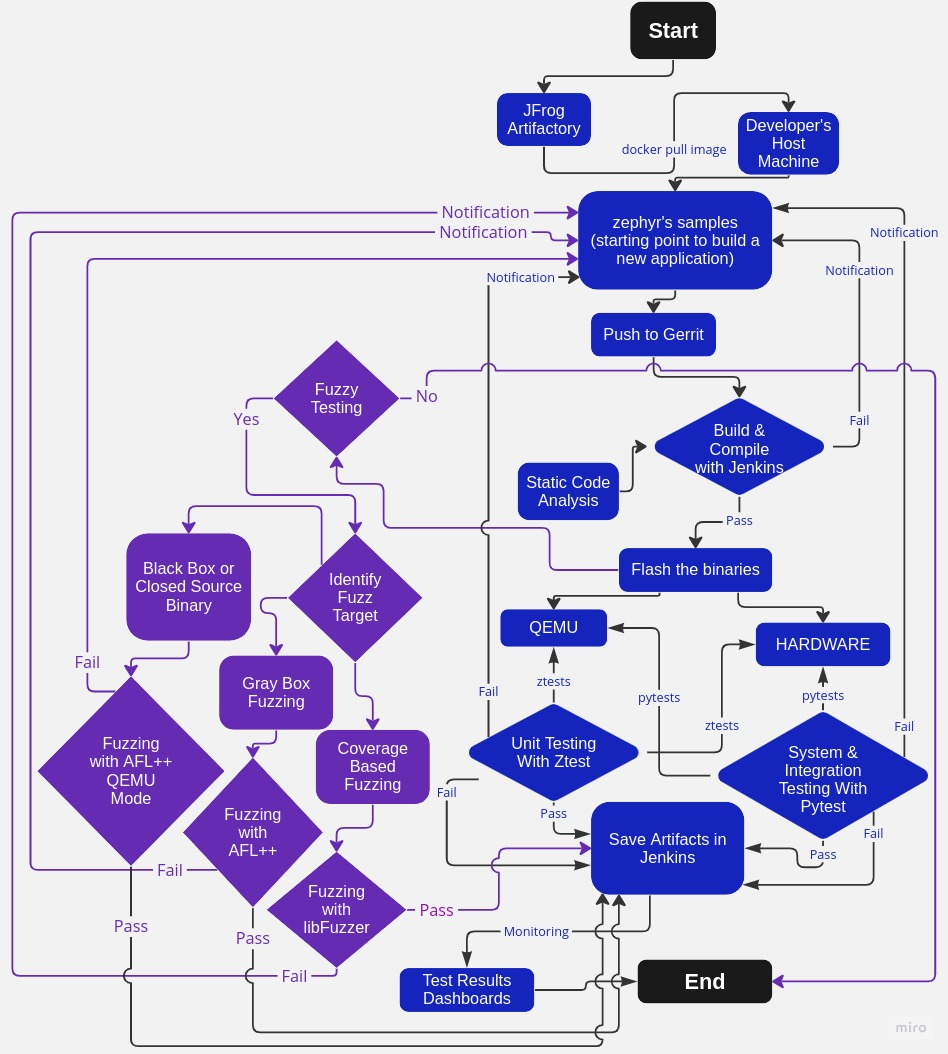
\includegraphics[width=\textwidth,height=0.8\textheight,keepaspectratio]{simplified_workflow_proposed}
\caption{Simplified Proposed Workflow}
\label{fig:simplified_workflow_proposed}
\end{figure}

\subsection*{Integration of Fuzzing}

Post the flashing of the firmware image~\cite{Firmware14:online}, an assessment
is undertaken to evaluate the compatibility of the binaries with fuzz testing, a process known as
``identifying the target'' in fuzz testing terminology and called as \gls{fuzz_target}.
This step is crucial for selecting the correct fuzz testing methodology.

Based on the characteristics of the \gls{fuzz_target}, various fuzz testing
methods are applicable. When the binary's compiler is identified, gray box
fuzzing~\cite{jamil2016software}, which strikes a balance between
blackbox'~\cite{godefroid2007random}~\cite{jamil2016software} and
whitebox'~\cite{godefroid2007random}~\cite{jamil2016software} fuzzing, should be
employed using afl-fuzz++~\cite{257204}. This approach encompasses
coverage-guided fuzzing~\cite{abran2001guide}, performed with
libfuzzer\cite{libFuzze17:online}. In contrast, if the binary's compiler is
unidentified, which is common with
black-box~\cite{jamil2016software}~\cite{pudas2017improving} or closed-source
binaries, the utilization of afl-fuzz in conjunction with QEMU is
advised~\cite{AFLplusp57:online}.

The enhanced workflow adds a supplementary layer of security
by methodically evaluating the software with a spectrum of unconventional
inputs. This process aids in pinpointing and mitigating potential
vulnerabilities before the software is deployed.

\begin{longtable}{p{1cm}p{3.7cm}p{3.7cm}p{3.7cm}}
\caption{Comparison of Current and Proposed System Workflows with Fuzzy Testing}
\label{tab:system_workflows_comparison_fuzzy} \\
\toprule
\textbf{Step} & \textbf{Current Workflow} & \textbf{Proposed Workflow} & \textbf{Changes and Notes} \\
\midrule
\endfirsthead

\toprule
\textbf{Step} & \textbf{Current Workflow} & \textbf{Proposed Workflow} & \textbf{Changes and Notes} \\
\midrule
\endhead

1 & Retrieve Docker Image from JFrog Artifactory & Retrieve Docker Image from JFrog Artifactory & No changes required \\
\midrule
2 & Develop sample application in Zephyr & Develop sample application in Zephyr & No changes required \\
\midrule
3 & Push to Gerrit for version control & Push to Gerrit for version control & No changes required \\
\midrule
4 & Compilation and building with Jenkins & Compilation and building with Jenkins & No changes required \\
\midrule
5 & Static code analysis with Jenkins & Static code analysis with Jenkins & No changes required \\
\midrule
6 & Flash binary images for both QEMU and hardware & Check eligibility for fuzz testing of the flashed binaries & Addition of a new step to determine eligibility for fuzz testing \\
\midrule
7 & Perform unit testing with ztest & Identify fuzz target based on eligibility & Addition of a new step for identifying the fuzz target \\
\midrule
8 & Conduct system and integration testing with pytest & Select appropriate fuzzing tools like AFL++, libFuzzer based on the target & Addition of a new step for selecting the appropriate fuzzing tool \\
\midrule
9 & Notification of failures & Validate the presence of bugs or vulnerabilities during unit, system, or fuzz testing & Addition of notifications for vulnerabilities identified during fuzz testing \\
\midrule
10 & Save test results in Artifactory & Record fuzz testing results & Addition of a new step to save the results of fuzz testing \\
\midrule
11 & Monitor test results & Monitor test results, including pass and fail ratios & Addition of monitoring for results of fuzz testing \\
\bottomrule
\end{longtable}


\subsection*{Benefits and Challenges:}
\textbf{Benefits:}~\cite{liang2018fuzz}~\cite{klees2018evaluating} \\
\begin{itemize}
    \item Enhances software security by proactively identifying and addressing vulnerabilities, thereby reducing risks associated with software exploits.
    \item Fosters the development of more resilient software, as developers become aware of potential issues and enhance their coding practices\cite{HowCICDI34:online}.
\end{itemize}

\textbf{Challenges:}~\cite{liang2018fuzz}~\cite{klees2018evaluating} \\
\begin{itemize}
    \item Resource-intensive, potentially extending the duration of the CI/CD pipeline.
    \item May yield false positives, necessitating additional time and resources to identify genuine vulnerabilities.
    \item Determining the appropriate times for conducting fuzz testing, such as off-peak hours or weekends.
    \item Establishing the optimal duration for fuzz testing.
    \item Managing test results, including logging failure conditions and steps to reproduce the issue~\cite{FuzzingC40:online}.
\end{itemize}


\clearpage